\pagebreak

\section{Situational Predictions}

Up until now, we've shown that time series predictions perform strictly better when using only non-zero data. However, when making our final prediction we can not simply ignore all contests that lack time series data before ``4 Hours Out''. To address this, we decided to use two distinct random forest ensembles: one including all Header, WLS and KF data and the other including only Header data. The first ensemble would then be used to predict on contests that have available time data and the second for those that don't. Figure \ref{fig:theSituation} shows the ROCs generated by following this situational predictive scheme.

\begin{figure}[h]
\centering
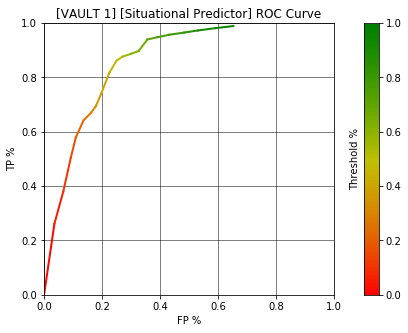
\includegraphics[width=8cm]{body/results/Graphs/SituationalPredictions/MetaWhenZero/v1.png}
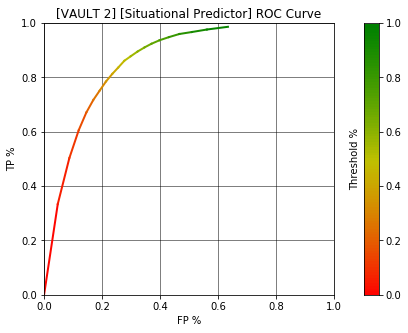
\includegraphics[width=8cm]{body/results/Graphs/SituationalPredictions/MetaWhenZero/v2.png}
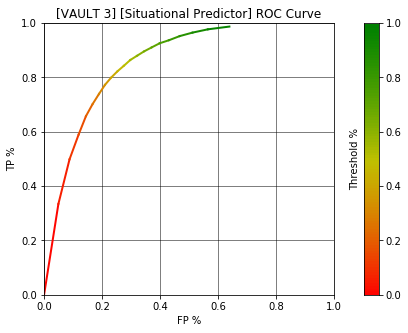
\includegraphics[width=8cm]{body/results/Graphs/SituationalPredictions/MetaWhenZero/v3.png}
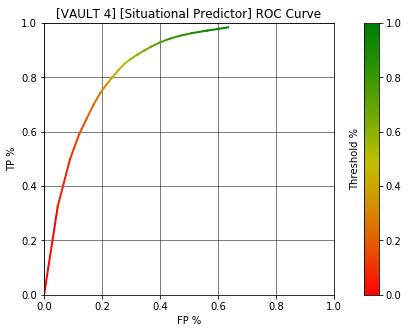
\includegraphics[width=8cm]{body/results/Graphs/SituationalPredictions/MetaWhenZero/v4.png}
\caption{ROCs generated based on the ensemble prediction of the outputs of all 15 of our WLS's and KF's (final entries prediction and model parameters) together on the entirety of each validation set and on just ``non-zero'' data. Top Left: Validation set 1. Top Right: Validation set 2. Bottom Left: Validation set 3. Bottom Right: Validation set 4.}
\label{fig:theSituation}
\end{figure}

\pagebreak

\begin{figure}[h]
\centering
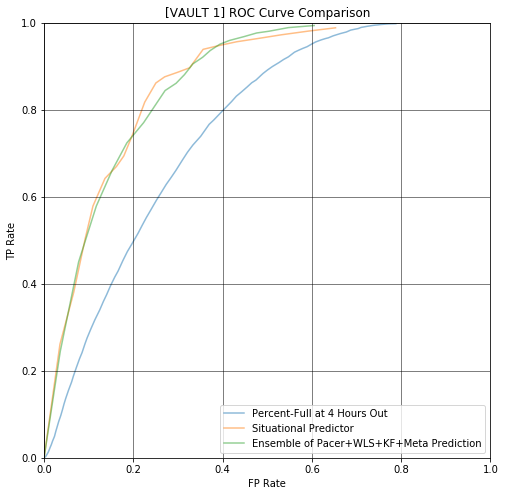
\includegraphics[width=7cm]{body/results/Graphs/SituationalPredictions/Compare/v1.png}
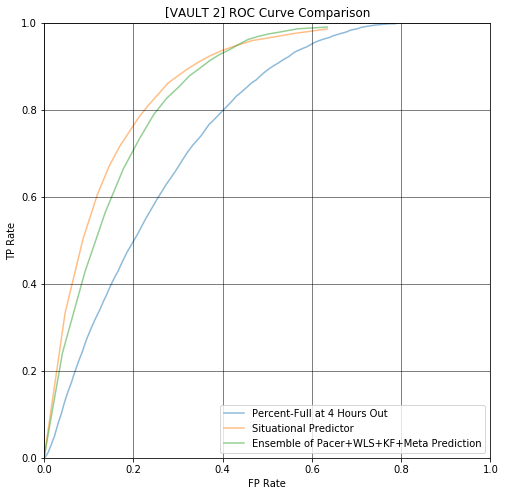
\includegraphics[width=7cm]{body/results/Graphs/SituationalPredictions/Compare/v2.png}
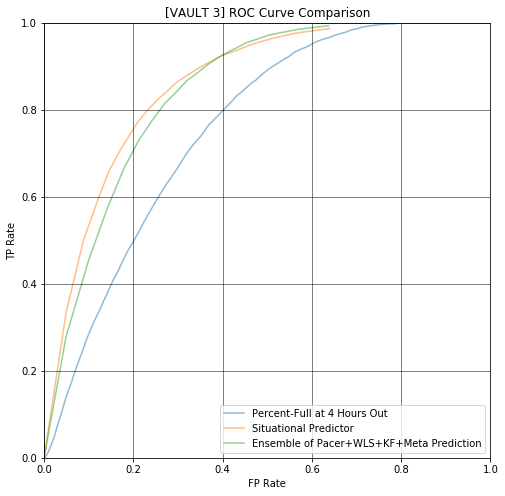
\includegraphics[width=7cm]{body/results/Graphs/SituationalPredictions/Compare/v3.png}
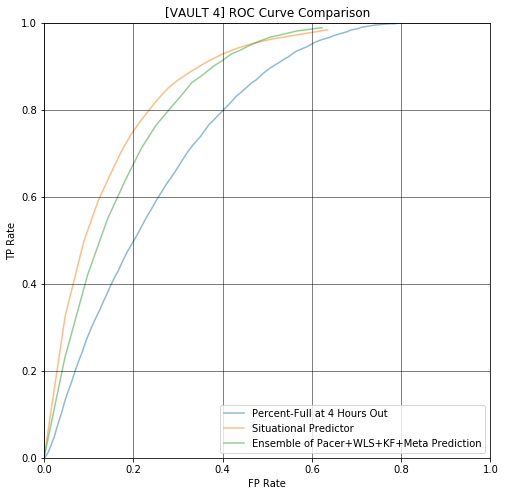
\includegraphics[width=7cm]{body/results/Graphs/SituationalPredictions/Compare/v4.png}
\caption{ROCs generated based on the ensemble prediction of the outputs of all 15 of our WLS's and KF's (final entries prediction and model parameters) together on the entirety of each validation set and on just ``non-zero'' data. Top Left: Validation set 1. Top Right: Validation set 2. Bottom Left: Validation set 3. Bottom Right: Validation set 4.}
\label{fig:SitComp}
\end{figure}

Figure \ref{fig:SitComp} shows a side by side comparison between using the situational predictor and using just the full ensemble. In all cases, we can see the situational predictor tends to outperform the full ensemble alone.